\begin{figure}[p]
	\centering

	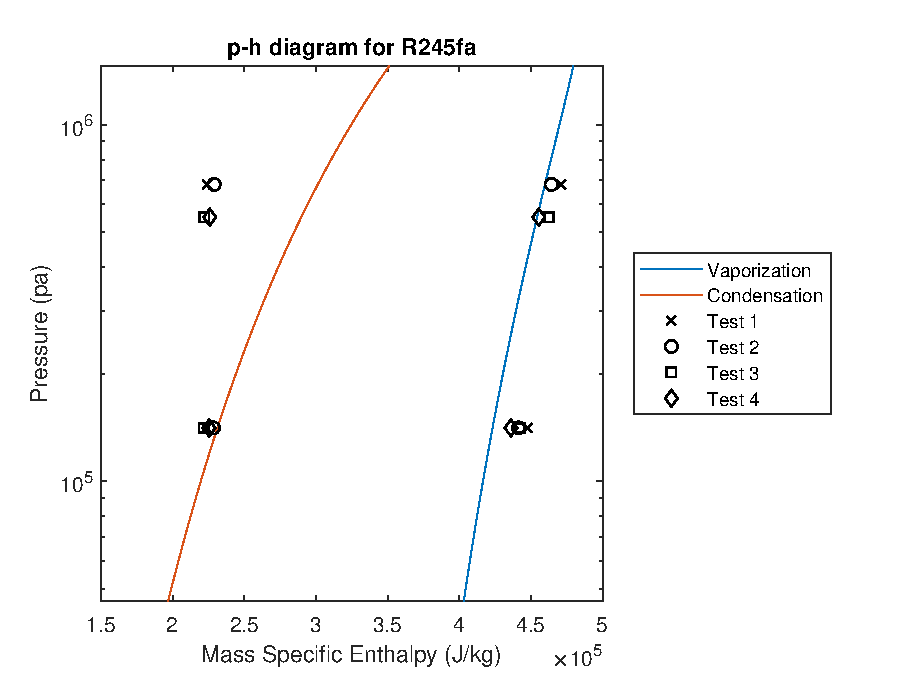
\includegraphics[width=\textwidth]{figures/VerificationPH02}
	%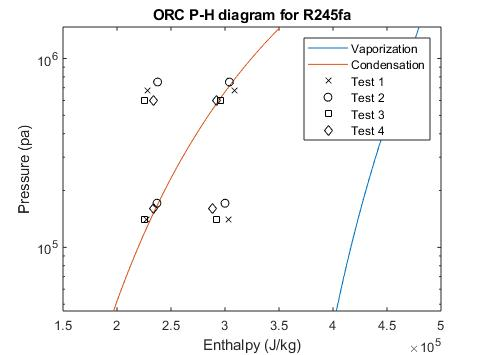
\includegraphics{figures/VerificationPH01}
	\caption{Pressure-mass specific enthalpy plot of R245-fa for ORC validation with an over sized evaporator area. Input temperatures and flow rates remain the same. 
	For tests 1 and 2 $T_{source\ in}$ is about \SI{364}{\kelvin} (\SI{91}{\degreeCelsius})
	while for tests 3 and 4 $T_{source\ in}$ is \SI{353}{\kelvin} (\SI{79}{\degreeCelsius}). 
	In all cases $T_{sink\ in}$ is about \SI{283}{\kelvin} (\SI{10}{\degreeCelsius}). 
	The hot water flow rate for tests 1 and 3 are \SI{18.9}{\liter\per\second} (\SI{300}{\gpm})
	and	\SI{7.6}{\liter\per\second} (\SI{120}{\gpm}) for tests 2 and 4. 
	The cold water flow rate for tests 1 and 3 are \SI{12.6}{\liter\per\second} (\SI{200}{\gpm})
	and \SI{7.6}{\liter\per\second} (\SI{120}{\gpm}) for tests 2 and 4.}
	\label{fig:verifcation_ph02}
\end{figure}